\documentclass[11pt,a4paper]{article}
\usepackage[utf8]{inputenc}
\usepackage[spanish]{babel}
\usepackage{amsmath}
\usepackage{amsfonts}
\usepackage{amssymb}
\usepackage{graphicx}
\usepackage[left=2cm,right=2cm,top=2cm,bottom=2cm]{geometry}
\title{\textbf{Universidad Politécnica de la Zona Metropolitana de Guadalajara
\\OptoAcopladores y relevadores
\\Sistemas Electrónicos de Interfaz}}
\begin{document}

\begin{center}
\begin{figure}
\begin{center}

\includegraphics[scale=1]{1.jpeg}
\end{center}
\end{figure}
\maketitle
\author{Barrera Vazquez Omar\\
Ing. Mecatrónica 4B}
\end{center}


\newpage

\section{Objetivos}
Trabajar con la aplicación de optoAcopldores y relevadores para la identificación de como se conforman las partes principales de un PLC y sus aplicaciones mas modestas.

\section{Materiales solicitados}
\begin{itemize}
\item 3 optoAcopladores
\item 3 resistencias de 1K$\Omega$
\item 3 resistencias cercanas a 15K$\Omega$
\item 2 leds rojos
\item 2 leds amarillos
\item 2 leds verdes
\item cable para Protoboard
\item fuente de alimentación 12 y 5 volts
\item 2 Protoboard
\item 1 placa del microprocesador ARDUINO
\item 3 relevadores de 5 volts
\item 3 transistores 2N2222
\item 3 resistencias de 670$\Omega$
\end{itemize}

\section{Modo de funcionamiento}
la realización de la practica llevada a cabo, es entender como funciona un PLC con sus partes básicas como los son; \emph{entradas, procesador y salidas} de esta manera al llevar a cabo la actividad se podrá entender el funcionamiento de control del PLC.

Las cuestiones a fundamentar son que es lo que necesita los \emph{optoAcopladores} para leer una señal de entrada y como es que el procesador interpreta esta señal y a su vez realiza una señal de salida también conocida como actuador.

\newpage

\section{Esquema de trabajo}
Para poder realizar la practica es necesario conocer el esquema que se va a trabajar y es el que se muestra a continuación:

\begin{center}
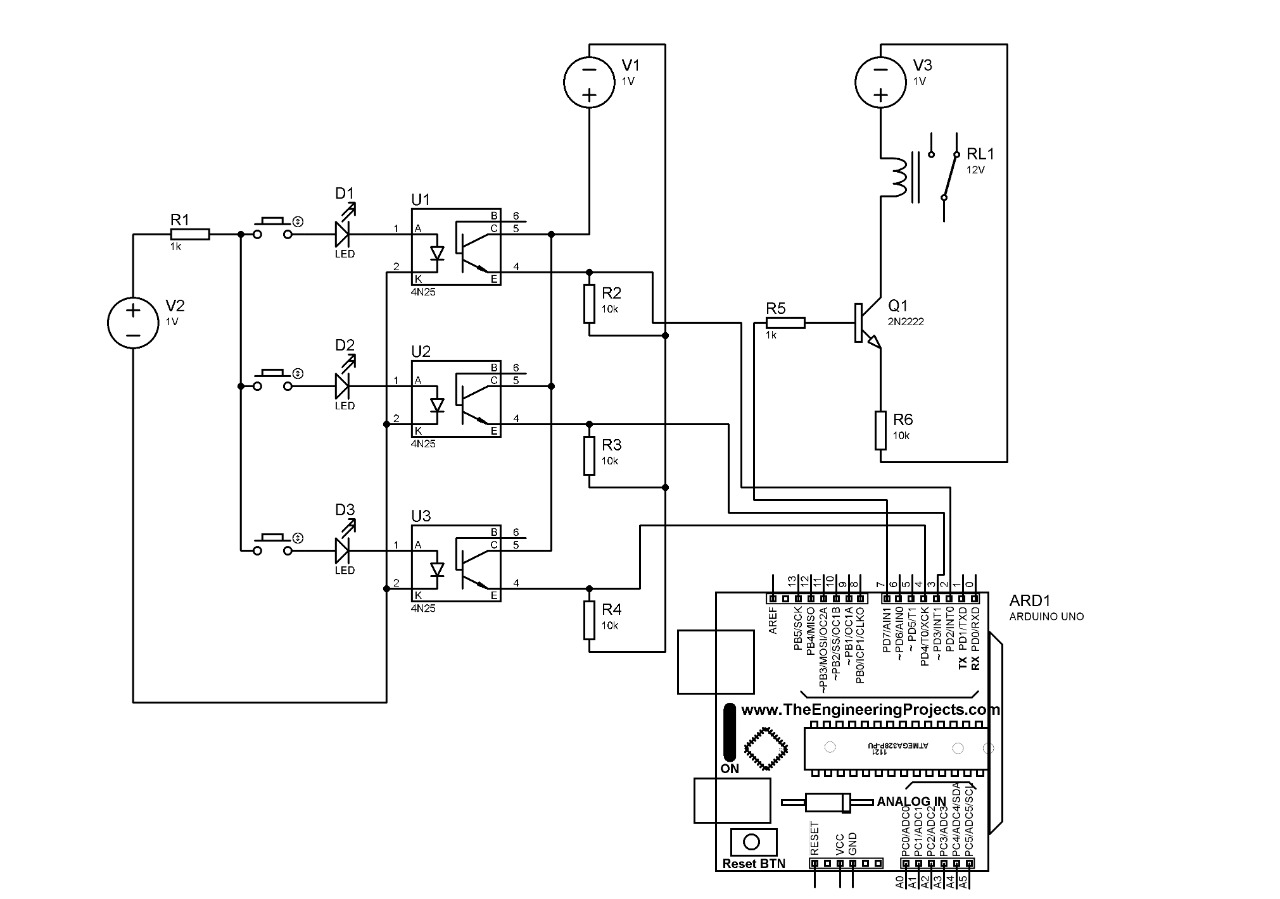
\includegraphics[scale=0.3]{2.jpeg}
\end{center}

En la figura anterior se observa como esta conformado un PLC, este lo conforman tres partes, divididas por el \emph{microprocesador} en este caso el arduino es nuestro procesador  por lo que la parte de los optoAcopladores es la parte de donde entraran las señales de lo que supuestamente son los sensores de un PLC llegaran estas señales en formas de 1 y 0 lógico al Arduino, el cual llevara a cabo el procesamiento lógico según las señales que obtenga de los sensores. Posteriormente tomara una decisión y enviara un señal de salida o respuesta, a lo que sera nuestro actuador, en nuestro caso sera un \emph{relevador que activara un algún aparato}. 

Anteriormente encontraremos lo que es un transistor modelo 2N2222 el cual nos ayudara a manejar el voltajes de nuestro actuador de manera independiente a la alimentación del procesador (Arduino). Tambien se puede agregar de manera paralela al relevador un \emph{diodo rectificador}, esto para evitar que una tension inversa llegara a dañar algún componente del nuestro circuito e incluso nuestro procesador.

\section{Elaboración del código en el procesador}
Para la elaboración del código en un PLC puede ser de distintas maneras, ya sea en formato \emph{ladder o Grafcet}, en este caso en particular se utilizo la programación de arduino, que aunque es un formato de programación sencillo y poco elaborado, tiene como las bases lógicas y de procesamiento para realizar procesos lógicos de baja demanda.

\subsection{Explicación del accionamiento del PLC}
En el sistema arduino realmente es muy fácil la realización de un código lógico solo se necesitan las siguientes acciones:
\begin{itemize}
\item en la primera parte se tiene que declarar la variable y definir el puerto, esto antes del void \emph{setup}
\item de manera posterior al \emph{setup} es necesario definir cuales puertos de los declarados serán entradas y cuales serán salidas
\item habiendo completado los pasos anteriores, es necesario dentro del \emph{void loop} empezar a trabajar con el código lógico, en este caso se utilizara el condicional lógico \textbf{if} 
\item dentro de los paréntesis se introducirá la condicional a realizar, y posteriormente al corchete la acción a realizar.

\end{itemize}

Se pueden basar una idea general de como funcionaria el código como el que se muestra a continuación:

\begin{center}
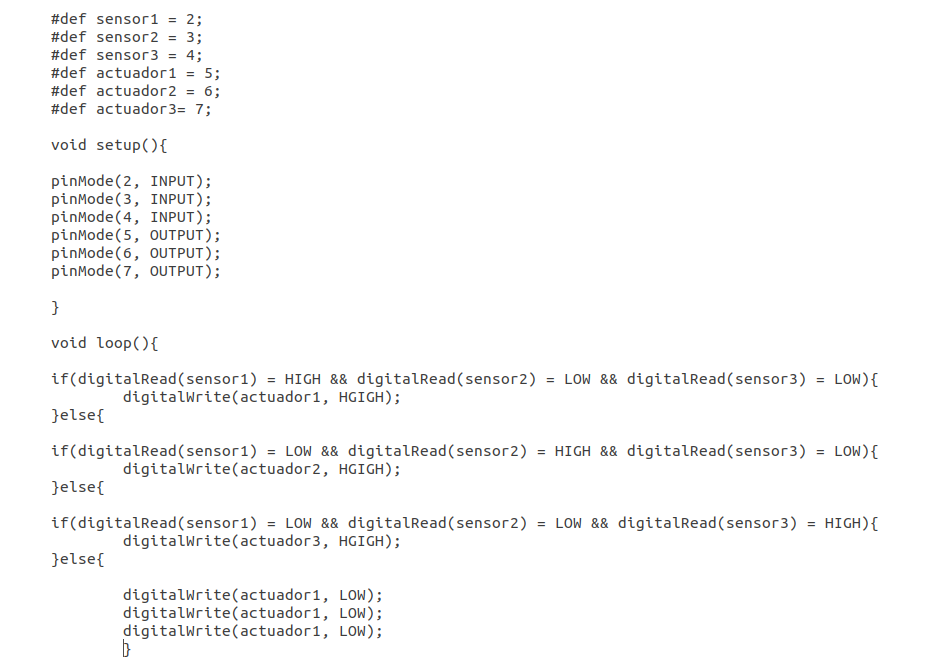
\includegraphics[scale=0.5]{3.png}
\end{center}


Una vez realizado el código solo es necesario cargar el código a la tarjeta arduino y esta tomara las decisiones en base al código introducido. Este código responde  a activar actuadores si su correspondiente sensor es activado, ejemplo: si el sensor 1 es activado lo correcto es que el actuador 1 sea activado, de esta forma es que se controlan diferentes encendidos y apagados de aparatos y luces.

los resultados mostrados son los que se muestran a continuación en la imagen:\\
\\
\\



\begin{figure}[h]
\begin{center}
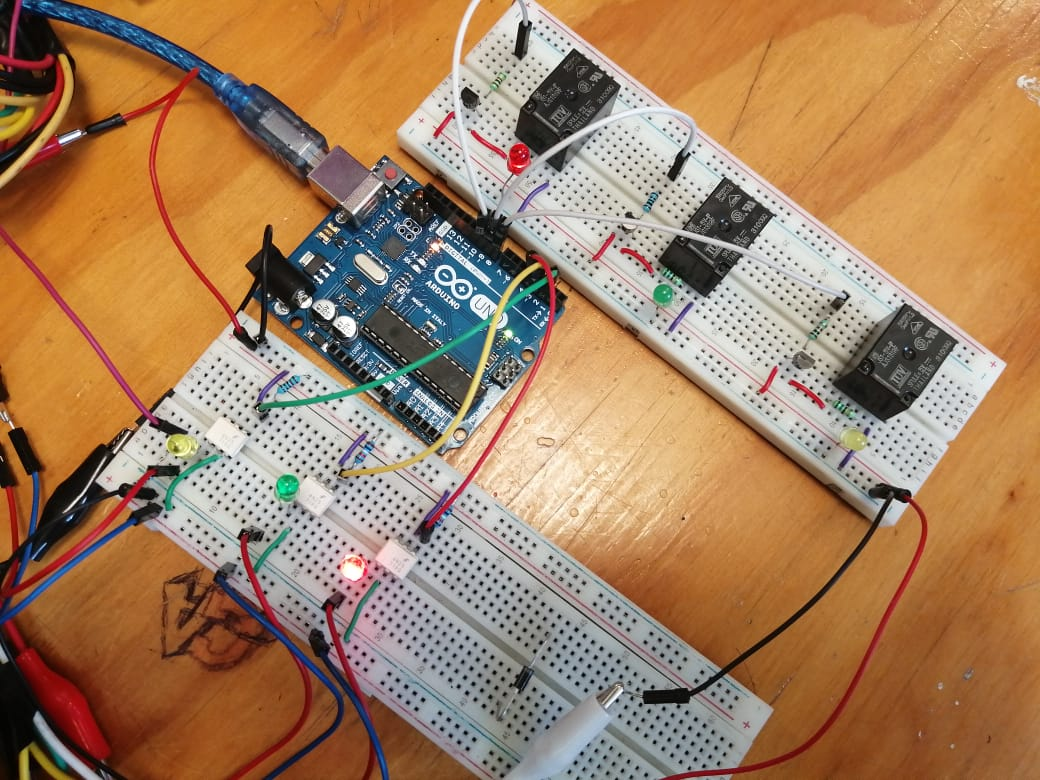
\includegraphics[scale=0.150]{5.jpeg}
\caption{sensor 2 actuador 2}
\end{center}
\end{figure}

\newpage

\section{Calculo de resistencias}

Parte de la practica consiste en realizar el calculo de la resistencia que antecede al optoAcoplador y al transistor 2N2222 los cuales deben tener una resistencia de protección ante una sobrecarga de tension, comenzaremos con obtener la resistencia adecuada para el optoAcoplador:


Teniendo presente la siguiente ecuación $P=\frac{V}{I}$ se observa que datos son los que se tienen para trabajar, sabemos que contamos con una tension de alimentación de \emph{12V}, y que la potencia máxima que resiste el optoAcoplador es de \emph{100mW}
 por que la formula anterior quedaría de la siguiente manera; $?P=12V*60mA$ por lo que la potencia a disipar de la resistencia es de 720mW por lo que tendrá que ser una resistencia de por lo menos $\frac{1}{2}$W ademas para obtener el valor de la resistencia solo es seguir la ley de ohm que es la siguiente formula $V=I*R$ entonces si se tienen los siguientes datos $12V=60mA*R$ solo se tiene que despejar la resistencia, por lo que la formula ya despejada quedaría de la siguiente manera $R=\frac{12V}{60mA}$ por lo que el valor de nuestra resistencia es la siguiente 200$\Omega$ esto sera el valor para cada entrada del circuito.
 
\section{Resultados de aprendizaje de la practica}

Aunque de manera sencilla y con determinados componentes eléctricos quedo representado la forma de un PLC podemos deducir lo siguiente:

\begin{itemize}
\item El PLC esta conformado por tres partes principales \emph{entrada de señal, procesador y salidas de señal}
\item La programación en PLC puede llegar a ser fácil, ya que ese es la idea de su formato, esto para que cualquier operario pueda interpretarlo
\item Con un PLC podemos controlar diferentes actuadores a través de uno o mas sensores

\end{itemize}

De esta manera concluye la practica sobre optoacopladore y relevadores en función de un PLC.





\end{document}